\documentclass{standalone}
\usepackage{tikz}
\usetikzlibrary{patterns, positioning}
\usepackage[sfdefault]{ClearSans} %% option 'sfdefault' activates Clear Sans as the default text font
\usepackage[T1]{fontenc}

\begin{document}
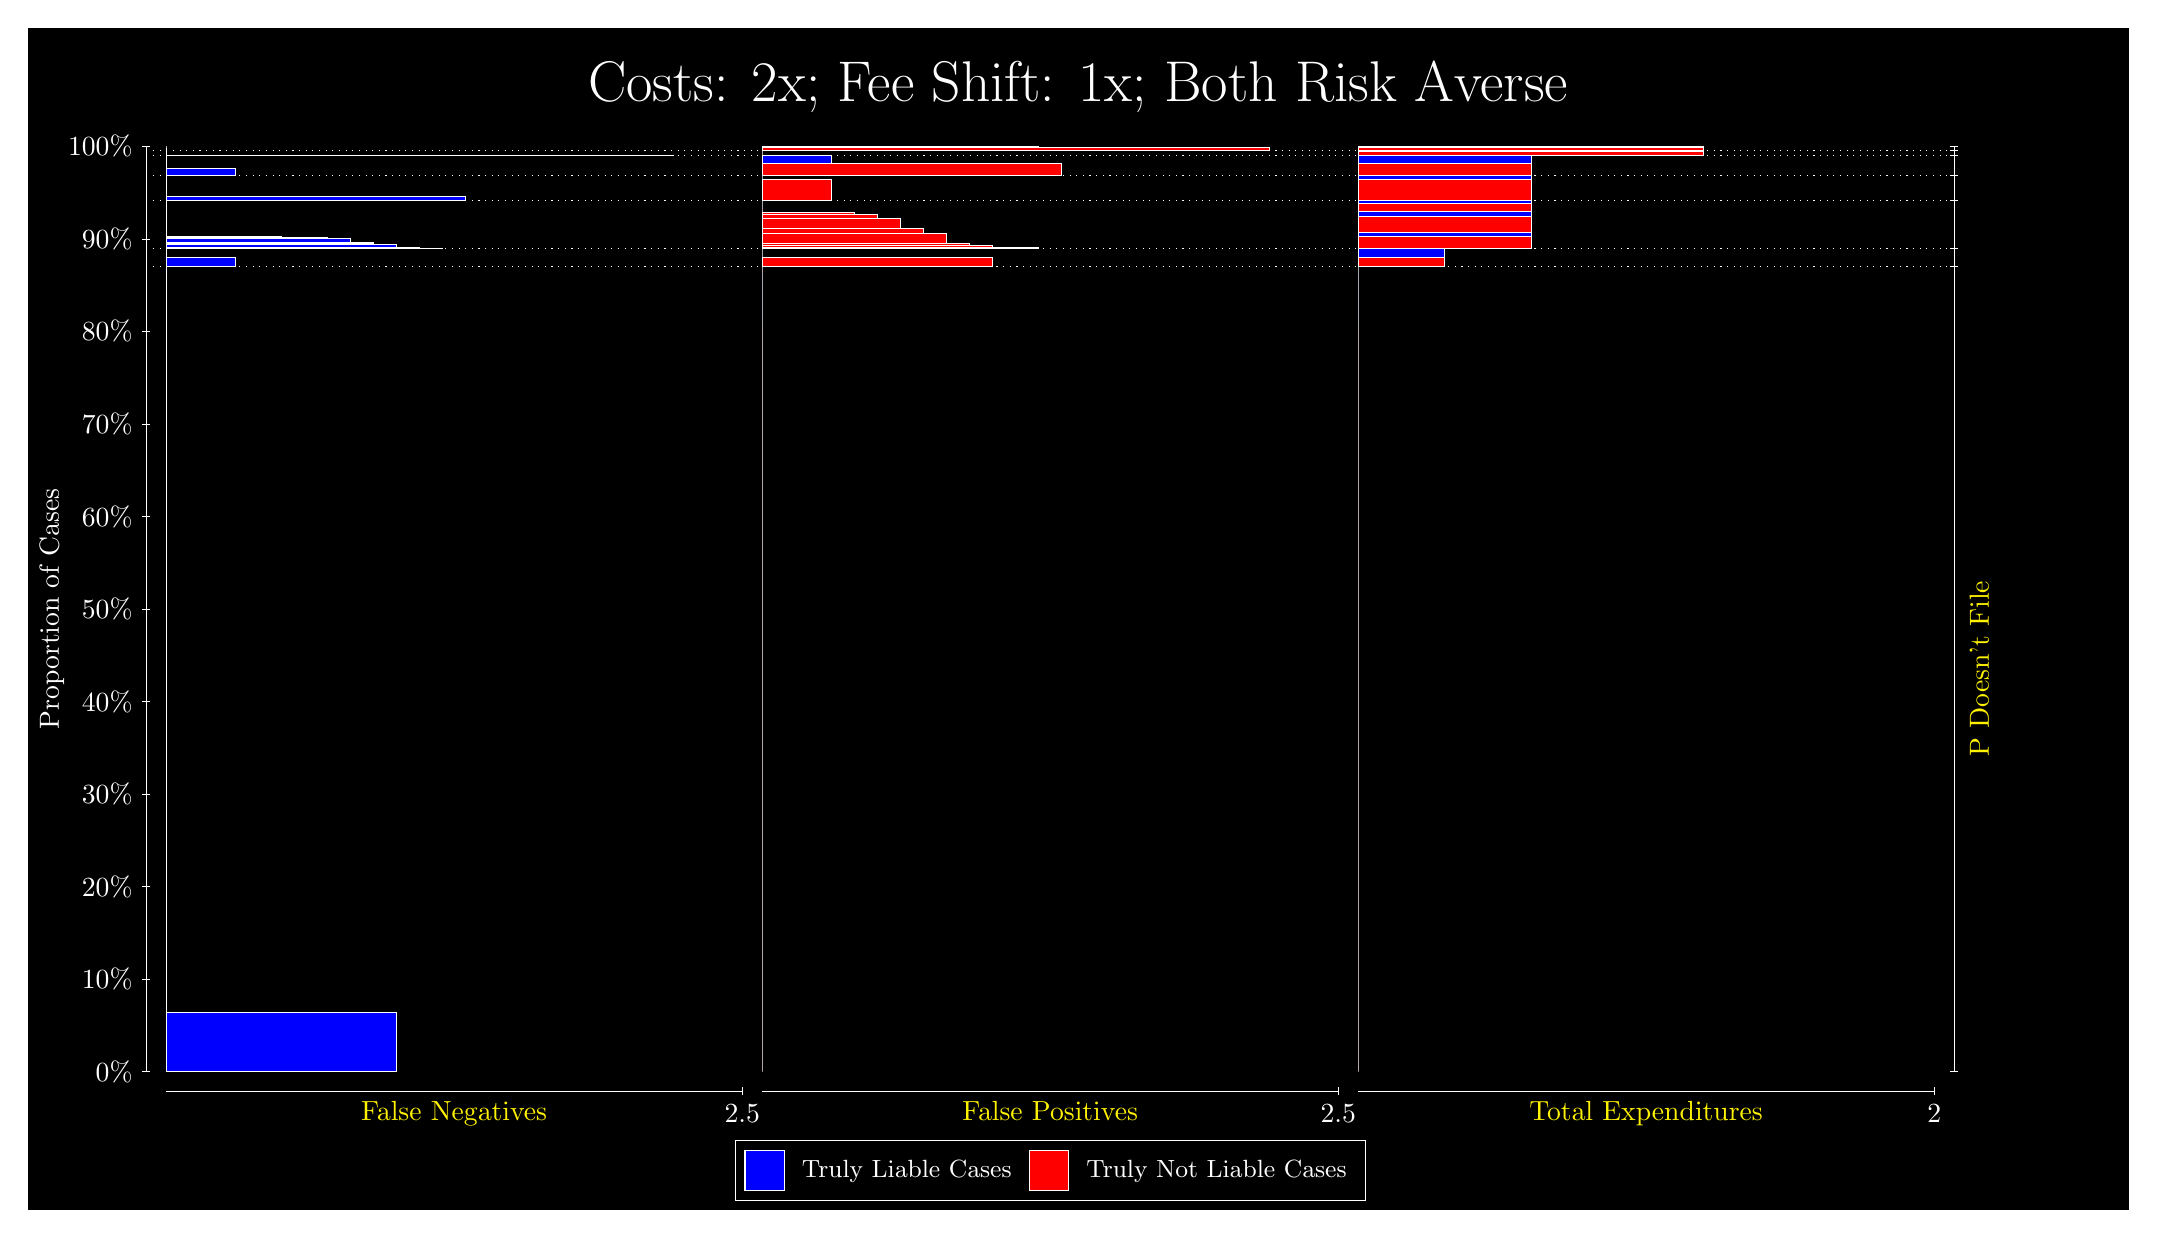
\begin{tikzpicture}
\draw[fill=black] (0,0) rectangle (26.667,15);
\draw[text=white] (0,13.5) rectangle (26.667,15) node[midway] {\huge Costs: 2x; Fee Shift: 1x; Both Risk Averse};
\draw[white, very thin] (1.5,1.75) -- (1.5,13.5);
\node[rotate=90, text=white, anchor=center] at (0.3, 7.625) {Proportion of Cases};
\draw[white, very thin] (1.45,1.75) -- (1.55,1.75);
\node[text=white, anchor=east] at (1.45, 1.75) {0\%};
\draw[white, very thin] (1.45,2.925) -- (1.55,2.925);
\node[text=white, anchor=east] at (1.45, 2.925) {10\%};
\draw[white, very thin] (1.45,4.1) -- (1.55,4.1);
\node[text=white, anchor=east] at (1.45, 4.1) {20\%};
\draw[white, very thin] (1.45,5.275) -- (1.55,5.275);
\node[text=white, anchor=east] at (1.45, 5.275) {30\%};
\draw[white, very thin] (1.45,6.45) -- (1.55,6.45);
\node[text=white, anchor=east] at (1.45, 6.45) {40\%};
\draw[white, very thin] (1.45,7.625) -- (1.55,7.625);
\node[text=white, anchor=east] at (1.45, 7.625) {50\%};
\draw[white, very thin] (1.45,8.8) -- (1.55,8.8);
\node[text=white, anchor=east] at (1.45, 8.8) {60\%};
\draw[white, very thin] (1.45,9.975) -- (1.55,9.975);
\node[text=white, anchor=east] at (1.45, 9.975) {70\%};
\draw[white, very thin] (1.45,11.15) -- (1.55,11.15);
\node[text=white, anchor=east] at (1.45, 11.15) {80\%};
\draw[white, very thin] (1.45,12.325) -- (1.55,12.325);
\node[text=white, anchor=east] at (1.45, 12.325) {90\%};
\draw[white, very thin] (1.45,13.5) -- (1.55,13.5);
\node[text=white, anchor=east] at (1.45, 13.5) {100\%};

\draw[white, very thin] (24.457,1.75) -- (24.457,13.5);
\draw[white, very thin] (24.407,1.75) -- (24.507,1.75);
\node[anchor=west] at (24.407, 1.75) {};
\draw[white, very thin] (24.407,11.978) -- (24.507,11.978);
\node[anchor=west] at (24.407, 11.978) {};
\draw[white, very thin] (24.407,12.204) -- (24.507,12.204);
\node[anchor=west] at (24.407, 12.204) {};
\draw[white, very thin] (24.407,12.812) -- (24.507,12.812);
\node[anchor=west] at (24.407, 12.812) {};
\draw[white, very thin] (24.407,13.132) -- (24.507,13.132);
\node[anchor=west] at (24.407, 13.132) {};
\draw[white, very thin] (24.407,13.381) -- (24.507,13.381);
\node[anchor=west] at (24.407, 13.381) {};
\draw[white, very thin] (24.407,13.444) -- (24.507,13.444);
\node[anchor=west] at (24.407, 13.444) {};
\draw[white, very thin] (24.407,13.5) -- (24.507,13.5);
\node[anchor=west] at (24.407, 13.5) {};

\draw[white, very thin, fill=blue] (1.75,1.75) rectangle (4.6775,2.4999);
\draw[white, very thin, fill=red] (1.75,2.4999) rectangle (1.75,11.978);
\draw[white, very thin, fill=blue] (1.75,11.978) rectangle (2.6283,12.085);
\draw[white, very thin, fill=red] (1.75,12.085) rectangle (1.75,12.204);
\draw[white, very thin, fill=blue] (1.75,12.204) rectangle (5.2631,12.208);
\draw[white, very thin, fill=blue] (1.75,12.208) rectangle (4.9703,12.223);
\draw[white, very thin, fill=blue] (1.75,12.223) rectangle (4.6775,12.261);
\draw[white, very thin, fill=blue] (1.75,12.261) rectangle (4.3848,12.263);
\draw[white, very thin, fill=blue] (1.75,12.263) rectangle (4.3848,12.287);
\draw[white, very thin, fill=blue] (1.75,12.287) rectangle (4.092,12.331);
\draw[white, very thin, fill=blue] (1.75,12.331) rectangle (3.7993,12.341);
\draw[white, very thin, fill=blue] (1.75,12.341) rectangle (3.5065,12.349);
\draw[white, very thin, fill=blue] (1.75,12.349) rectangle (3.2138,12.352);
\draw[white, very thin, fill=blue] (1.75,12.352) rectangle (2.921,12.356);
\draw[white, very thin, fill=red] (1.75,12.356) rectangle (1.75,12.812);
\draw[white, very thin, fill=blue] (1.75,12.812) rectangle (5.5558,12.863);
\draw[white, very thin, fill=red] (1.75,12.863) rectangle (1.75,13.132);
\draw[white, very thin, fill=blue] (1.75,13.132) rectangle (2.6283,13.223);
\draw[white, very thin, fill=red] (1.75,13.223) rectangle (1.75,13.381);
\draw[white, very thin, fill=blue] (1.75,13.381) rectangle (8.1906,13.385);
\draw[white, very thin, fill=red] (1.75,13.385) rectangle (1.75,13.444);
\draw[white, very thin, fill=red] (1.75,13.444) rectangle (1.75,13.482);
\draw[white, very thin, fill=blue] (1.75,13.482) rectangle (1.75,13.5);
\draw[white, very thin, fill=red] (9.3189,1.75) rectangle (9.3189,11.228);
\draw[white, very thin, fill=blue] (9.3189,11.228) rectangle (9.3189,11.978);
\draw[white, very thin, fill=red] (9.3189,11.978) rectangle (12.246,12.096);
\draw[white, very thin, fill=blue] (9.3189,12.096) rectangle (9.3189,12.204);
\draw[white, very thin, fill=red] (9.3189,12.204) rectangle (12.832,12.213);
\draw[white, very thin, fill=red] (9.3189,12.213) rectangle (12.539,12.22);
\draw[white, very thin, fill=red] (9.3189,12.22) rectangle (12.246,12.244);
\draw[white, very thin, fill=red] (9.3189,12.244) rectangle (11.954,12.273);
\draw[white, very thin, fill=red] (9.3189,12.273) rectangle (11.661,12.39);
\draw[white, very thin, fill=red] (9.3189,12.39) rectangle (11.368,12.462);
\draw[white, very thin, fill=red] (9.3189,12.462) rectangle (11.075,12.587);
\draw[white, very thin, fill=red] (9.3189,12.587) rectangle (10.783,12.634);
\draw[white, very thin, fill=red] (9.3189,12.634) rectangle (10.49,12.66);
\draw[white, very thin, fill=blue] (9.3189,12.66) rectangle (9.9044,12.664);
\draw[white, very thin, fill=blue] (9.3189,12.664) rectangle (9.6116,12.667);
\draw[white, very thin, fill=blue] (9.3189,12.667) rectangle (9.3189,12.812);
\draw[white, very thin, fill=red] (9.3189,12.812) rectangle (10.197,13.08);
\draw[white, very thin, fill=blue] (9.3189,13.08) rectangle (9.3189,13.132);
\draw[white, very thin, fill=red] (9.3189,13.132) rectangle (13.125,13.289);
\draw[white, very thin, fill=blue] (9.3189,13.289) rectangle (10.197,13.381);
\draw[white, very thin, fill=red] (9.3189,13.381) rectangle (9.3189,13.44);
\draw[white, very thin, fill=blue] (9.3189,13.44) rectangle (9.3189,13.444);
\draw[white, very thin, fill=red] (9.3189,13.444) rectangle (15.759,13.482);
\draw[white, very thin, fill=blue] (9.3189,13.482) rectangle (12.832,13.5);
\draw[white, very thin, fill=red] (16.888,1.75) rectangle (16.888,11.228);
\draw[white, very thin, fill=blue] (16.888,11.228) rectangle (16.888,11.978);
\draw[white, very thin, fill=red] (16.888,11.978) rectangle (17.986,12.096);
\draw[white, very thin, fill=blue] (16.888,12.096) rectangle (17.986,12.204);
\draw[white, very thin, fill=red] (16.888,12.204) rectangle (19.083,12.352);
\draw[white, very thin, fill=blue] (16.888,12.352) rectangle (19.083,12.408);
\draw[white, very thin, fill=red] (16.888,12.408) rectangle (19.083,12.612);
\draw[white, very thin, fill=blue] (16.888,12.612) rectangle (19.083,12.671);
\draw[white, very thin, fill=red] (16.888,12.671) rectangle (19.083,12.774);
\draw[white, very thin, fill=blue] (16.888,12.774) rectangle (19.083,12.812);
\draw[white, very thin, fill=red] (16.888,12.812) rectangle (19.083,13.08);
\draw[white, very thin, fill=blue] (16.888,13.08) rectangle (19.083,13.132);
\draw[white, very thin, fill=red] (16.888,13.132) rectangle (19.083,13.289);
\draw[white, very thin, fill=blue] (16.888,13.289) rectangle (19.083,13.381);
\draw[white, very thin, fill=red] (16.888,13.381) rectangle (21.279,13.44);
\draw[white, very thin, fill=blue] (16.888,13.44) rectangle (21.279,13.444);
\draw[white, very thin, fill=red] (16.888,13.444) rectangle (21.279,13.482);
\draw[white, very thin, fill=blue] (16.888,13.482) rectangle (21.279,13.5);
\draw[white, dotted] (1.5,11.978) -- (24.457,11.978);
\draw[white, dotted] (1.5,12.204) -- (24.457,12.204);
\draw[white, dotted] (1.5,12.812) -- (24.457,12.812);
\draw[white, dotted] (1.5,13.132) -- (24.457,13.132);
\draw[white, dotted] (1.5,13.381) -- (24.457,13.381);
\draw[white, dotted] (1.5,13.444) -- (24.457,13.444);
\draw[white, very thin] (1.75,1.5) -- (9.0689,1.5);
\node[text=yellow, anchor=north] at (5.4094, 1.5) {False Negatives};
\draw[white, very thin] (9.0689,1.45) -- (9.0689,1.55);
\node[text=white, anchor=north] at (9.0689, 1.45) {2.5};

\draw[white, very thin] (9.3189,1.5) -- (16.638,1.5);
\node[text=yellow, anchor=north] at (12.978, 1.5) {False Positives};
\draw[white, very thin] (16.638,1.45) -- (16.638,1.55);
\node[text=white, anchor=north] at (16.638, 1.45) {2.5};

\draw[white, very thin] (16.888,1.5) -- (24.207,1.5);
\node[text=yellow, anchor=north] at (20.547, 1.5) {Total Expenditures};
\draw[white, very thin] (24.207,1.45) -- (24.207,1.55);
\node[text=white, anchor=north] at (24.207, 1.45) {2};

\node[text=yellow, centered, rotate=90] at (24.777, 6.8639) {P Doesn't File};







\draw (12.978300999999998,1.5) node[draw=none] (baseCoordinate) {};
\begin{scope}[align=center]
        \matrix[scale=0.5, draw=white, below=0.5cm of baseCoordinate, nodes={draw}, column sep=0.1cm]{
            \node[rectangle, draw, minimum width=0.5cm, minimum height=0.5cm, fill=blue] {}; &
            \node[draw=none, font=\small, text=white] (B) {Truly Liable Cases}; &
            \node[rectangle, draw, minimum width=0.5cm, minimum height=0.5cm, fill=red] {}; &
            \node[draw=none, font=\small, text=white] (B) {Truly Not Liable Cases}; \\
            };
\end{scope}

\end{tikzpicture}
\end{document}